\subsection{Electric Pathways: Parallel Conductors vs. Coaxial Cables!}

\begin{tcolorbox}[colback=gray!10, colframe=black, title=E9F07]
How does parallel conductor transmission line compare to coaxial cable with a plastic dielectric? 
\begin{enumerate}[label=\Alph*.]
    \item Lower loss
    \item Higher SWR
    \item Smaller reflection coefficient
    \item Lower velocity factor
\end{enumerate} \end{tcolorbox}

The correct answer is: \textbf{A}.

\subsubsection{Related Concepts}

To understand the differences between parallel conductor transmission lines and coaxial cables, we must consider several concepts in radio communication and electronics, including impedance, loss characteristics, standing wave ratio (SWR), reflection coefficient, and velocity factor.

1. \textbf{Impedance:}: Coaxial cables generally have a fixed characteristic impedance (often 50 or 75 ohms), which is particularly important in RF applications to ensure maximum power transfer and minimal reflections. In contrast, the impedance of a parallel conductor transmission line can vary based on the spacing between the conductors and their geometry.

2. \textbf{Loss Characteristics:}: 
   - Parallel conductor lines tend to have higher resistive losses at high frequencies due to the increased skin effect and potential radiation losses.
   - Coaxial cables typically exhibit lower losses due to the more efficient dielectric surrounding the inner conductor, which can maintain higher signal strength over long distances.

3. \textbf{Standing Wave Ratio (SWR):}: This is a measure of impedance matching in transmission lines. Coaxial cables are designed to maintain better SWR due to their consistent characteristic impedance. In contrast, parallel conductors may experience higher SWR due to variations in their effective impedance, especially if not properly configured.

4. \textbf{Reflection Coefficient:}: The reflection coefficient quantifies how much of a wave is reflected back when it encounters an impedance mismatch. Coaxial cables produce a smaller reflection coefficient compared to parallel conductor lines, further optimizing signal integrity.

5. \textbf{Velocity Factor:}: This term refers to the speed at which a signal travels through a transmission medium relative to the speed of light. Coaxial cables have a higher velocity factor compared to parallel conductor transmission lines because of the insulation material used, which allows signals to propagate faster.

\subsubsection{Calculation Steps (Optional)}

While no direct calculation is presented in this question, if one were to compare the loss characteristics mathematically, one would typically analyze the insertion loss using the formulas specific to each type of transmission line. For instance, the insertion loss (\(L\)) can be calculated using:

\[
L = 10 \log_{10} \left( \frac{P_{in}}{P_{out}} \right)
\]

Where \(P_{in}\) is the input power and \(P_{out}\) is the output power after transmission through the line. If the insertion loss of coaxial cable is found to be significantly less than that of a parallel conductor line, it would confirm that coaxial cables provide lower loss.

\subsubsection{Diagram Representation}

To visualize the difference, we can represent the structures of the transmission lines using TikZ. Below is a simple representation of both types of transmission lines:

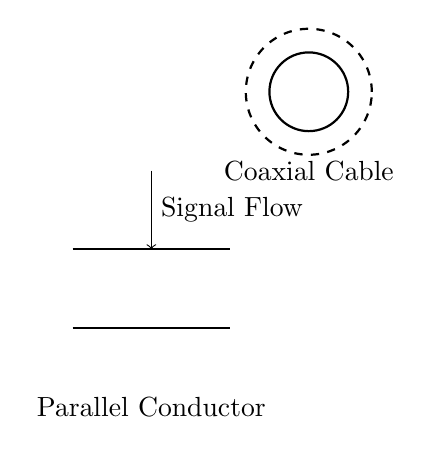
\begin{tikzpicture}
    % Coaxial Cable
    \draw[thick] (0,0) circle(0.5);
    \draw[thick, dashed] (0,0) circle(0.8);
    \node at (0,-1) {Coaxial Cable};
 
    % Parallel Conductor
    \draw[thick] (-3,-2) -- (-1,-2);
    \draw[thick] (-3,-3) -- (-1,-3);
    \node at (-2,-4) {Parallel Conductor};

    \draw[->] (-2,-1) -- (-2,-2) node[midway,right] {Signal Flow};
\end{tikzpicture}

In summary, the parallel conductor transmission line tends to have lower loss compared to coaxial cables due to its construction and the characteristics of the dielectric. This is a crucial aspect for applications in RF communication and signals transport.
